\documentclass[14pt,xcolor=pdftex,dvipsnames,table]{beamer}\usepackage{graphicx, color}
%% maxwidth is the original width if it is less than linewidth
%% otherwise use linewidth (to make sure the graphics do not exceed the margin)
\makeatletter
\def\maxwidth{ %
  \ifdim\Gin@nat@width>\linewidth
    \linewidth
  \else
    \Gin@nat@width
  \fi
}
\makeatother

\definecolor{fgcolor}{rgb}{0.2, 0.2, 0.2}
\newcommand{\hlnumber}[1]{\textcolor[rgb]{0,0,0}{#1}}%
\newcommand{\hlfunctioncall}[1]{\textcolor[rgb]{0.501960784313725,0,0.329411764705882}{\textbf{#1}}}%
\newcommand{\hlstring}[1]{\textcolor[rgb]{0.6,0.6,1}{#1}}%
\newcommand{\hlkeyword}[1]{\textcolor[rgb]{0,0,0}{\textbf{#1}}}%
\newcommand{\hlargument}[1]{\textcolor[rgb]{0.690196078431373,0.250980392156863,0.0196078431372549}{#1}}%
\newcommand{\hlcomment}[1]{\textcolor[rgb]{0.180392156862745,0.6,0.341176470588235}{#1}}%
\newcommand{\hlroxygencomment}[1]{\textcolor[rgb]{0.43921568627451,0.47843137254902,0.701960784313725}{#1}}%
\newcommand{\hlformalargs}[1]{\textcolor[rgb]{0.690196078431373,0.250980392156863,0.0196078431372549}{#1}}%
\newcommand{\hleqformalargs}[1]{\textcolor[rgb]{0.690196078431373,0.250980392156863,0.0196078431372549}{#1}}%
\newcommand{\hlassignement}[1]{\textcolor[rgb]{0,0,0}{\textbf{#1}}}%
\newcommand{\hlpackage}[1]{\textcolor[rgb]{0.588235294117647,0.709803921568627,0.145098039215686}{#1}}%
\newcommand{\hlslot}[1]{\textit{#1}}%
\newcommand{\hlsymbol}[1]{\textcolor[rgb]{0,0,0}{#1}}%
\newcommand{\hlprompt}[1]{\textcolor[rgb]{0.2,0.2,0.2}{#1}}%

\usepackage{framed}
\makeatletter
\newenvironment{kframe}{%
 \def\at@end@of@kframe{}%
 \ifinner\ifhmode%
  \def\at@end@of@kframe{\end{minipage}}%
  \begin{minipage}{\columnwidth}%
 \fi\fi%
 \def\FrameCommand##1{\hskip\@totalleftmargin \hskip-\fboxsep
 \colorbox{shadecolor}{##1}\hskip-\fboxsep
     % There is no \\@totalrightmargin, so:
     \hskip-\linewidth \hskip-\@totalleftmargin \hskip\columnwidth}%
 \MakeFramed {\advance\hsize-\width
   \@totalleftmargin\z@ \linewidth\hsize
   \@setminipage}}%
 {\par\unskip\endMakeFramed%
 \at@end@of@kframe}
\makeatother

\definecolor{shadecolor}{rgb}{.97, .97, .97}
\definecolor{messagecolor}{rgb}{0, 0, 0}
\definecolor{warningcolor}{rgb}{1, 0, 1}
\definecolor{errorcolor}{rgb}{1, 0, 0}
\newenvironment{knitrout}{}{} % an empty environment to be redefined in TeX

\usepackage{alltt}

% Specify theme
\usetheme{Madrid}
% See deic.uab.es/~iblanes/beamer_gallery/index_by_theme.html for other themes
\usepackage{caption}
\usepackage[comma, sort&compress]{natbib}
\usepackage{graphicx}
\usepackage{amsmath}
\bibliographystyle{agsm}
% Specify base color
\usecolortheme[named=OliveGreen]{structure}
% See http://goo.gl/p0Phn for other colors

% Specify other colors and options as required
\setbeamercolor{alerted text}{fg=Maroon}
\setbeamertemplate{items}[square]

% Title and author information
\title{Pairs Trading - Relative Value}
\author{Rob Hayward}
\IfFileExists{upquote.sty}{\usepackage{upquote}}{}


\begin{document}

\begin{frame}
\titlepage
\end{frame}

\begin{frame}{Outline}
\tableofcontents
\end{frame}

\section{Introduction}
\begin{frame}{Introduction}
This is a return full circle to the original hedge funds
\begin{itemize}[<+-| alert@+>]
\item Pairs trading will hope to provide an \emph{absolute return}
\item Paris trading can remove market risk and leave exposure to specific risk
\item Depends upon being able to short securities
\begin{itemize}
\item Professional ability to borrow securities
\item Use futures or contract-for-difference
\end{itemize}
\end{itemize}
\end{frame}

\section{Pairs Trading}
\begin{frame}{Pairs Trading}
The trade depends on a temporary breakdown in the correlation between two similar securities
\begin{itemize}[<+-| alert@+>]
\item LTCM strategy
\item When the usual relationship breaks down, speculate on a return to normality
\item Examples
\begin{itemize}
\item Tesco and Sainsbury
\item Coke and Pepsi
\item 5-year bond and 10-year bond
\item Gold and silver
\end{itemize}
\end{itemize}
\end{frame}

\begin{frame}{Pairs}
\begin{knitrout}
\definecolor{shadecolor}{rgb}{0.969, 0.969, 0.969}\color{fgcolor}
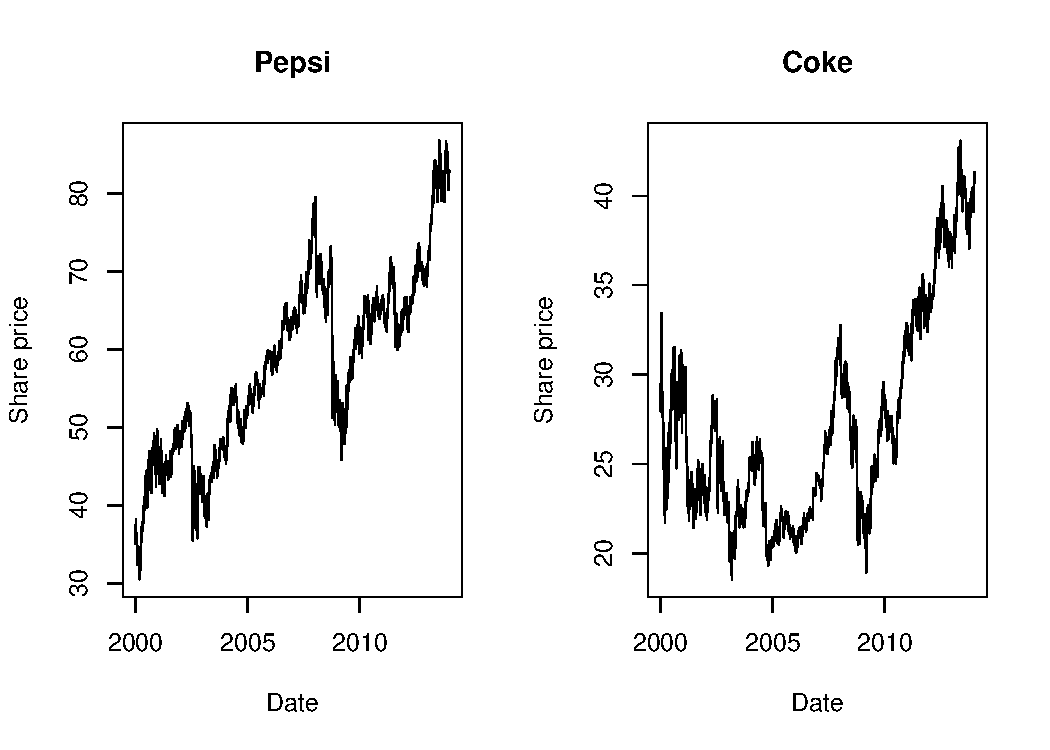
\includegraphics[width=\maxwidth]{figure/Coke} 

\end{knitrout}

\end{frame}

\begin{frame}{Coke vs Pepsi}
\begin{knitrout}
\definecolor{shadecolor}{rgb}{0.969, 0.969, 0.969}\color{fgcolor}
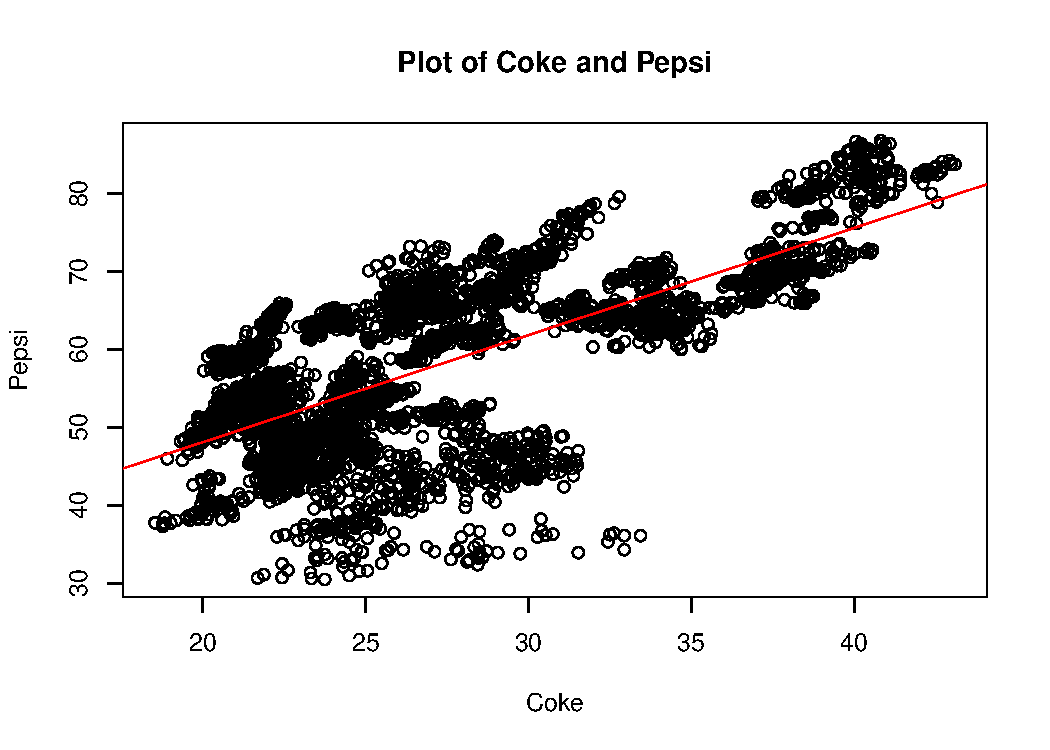
\includegraphics[width=\maxwidth]{figure/Coke2} 

\end{knitrout}

\end{frame}

\begin{frame}{Coke vs Pepsi}
\begin{knitrout}
\definecolor{shadecolor}{rgb}{0.969, 0.969, 0.969}\color{fgcolor}
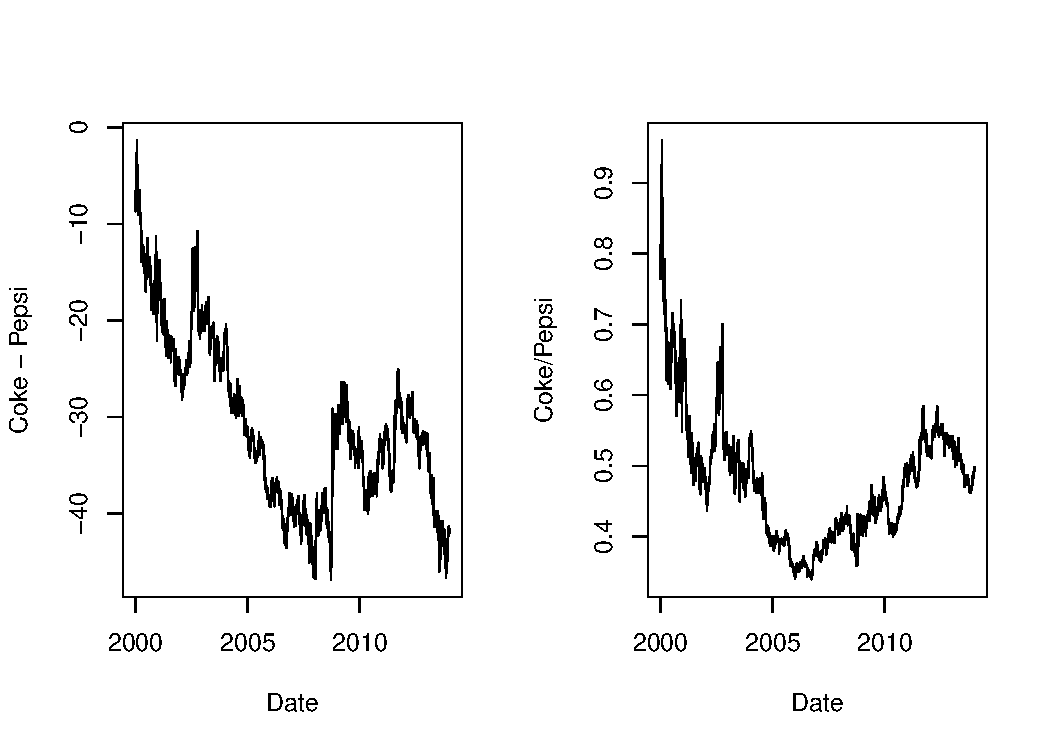
\includegraphics[width=\maxwidth]{figure/CvP} 

\end{knitrout}

\end{frame}

\begin{frame}{Cointegration}
One method to look at the relationship would be the assess whether the two are cointegrated.
\begin{itemize}[<+-| alert@+>]
\item Can use the Engle-Granger method and check that the residuals from the regression are \emph{stationary}
\item If the residuals are stationary, we expect the previous relationship to be restored
\item An \emph{Error-Correction Model} can be used to assess the speed of the return to the set relationship
\end{itemize}
\end{frame}
%\begin{frame}{OLS Coke and Pepsi}
%<<table>>=
%xtable(summary(eq))
%@
%\end{frame}
% This does not work.  
\begin{frame}{Regression: Coke and Pepsi}
% latex table generated in R 3.0.2 by xtable 1.7-1 package
% Fri Mar 21 05:51:48 2014
\begin{table}[ht]
\rowcolors{1}{OliveGreen!20}{OliveGreen!5}
\centering
\begin{tabular}{rrrrr}
  \hline
 & Estimate & Std. Error & t value & Pr($>$$|$t$|$) \\ 
  \hline
(Intercept) & 20.58 & 0.68 & 30.16 & 0.00 \\ 
  Coke & 1.37 & 0.02 & 56.18 & 0.00 \\ 
   \hline
\end{tabular}
\end{table}

The regression of Pepsi on Cole is only valid if the two are cointegrated.  Residuals must be checked. 

\end{frame}

\begin{frame}{Residuals}
\begin{knitrout}
\definecolor{shadecolor}{rgb}{0.969, 0.969, 0.969}\color{fgcolor}
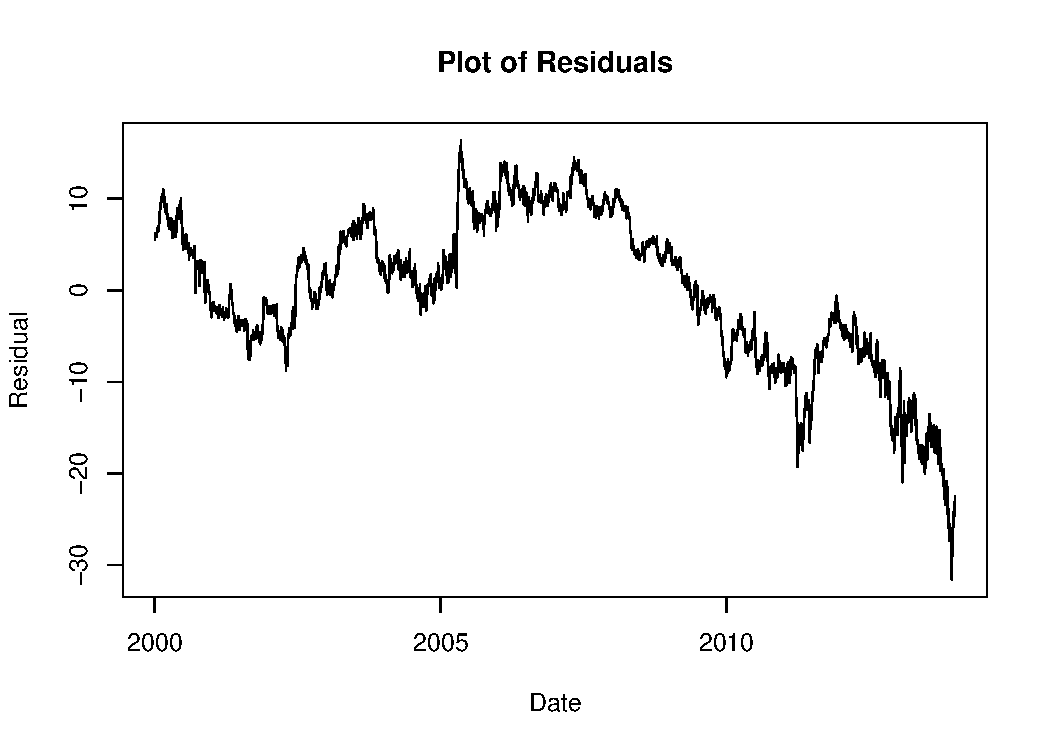
\includegraphics[width=\maxwidth]{figure/Resid} 

\end{knitrout}

\end{frame}

%<<DF, echo=FALSE, message=FALSE>>=
%require(urca)
%da4 <- ur.df(eq$residuals, type = 'trend', lags = 3) 
%# Does not print anything.  the table is manual
%@
\begin{frame}{Dickey-Fuller}
\begin{table}[ht]
\rowcolors{1}{OliveGreen!20}{OliveGreen!5}
\centering
\begin{tabular}{rrrr}
  \hline
   & Test & 1pct& 5pct  \\ 
  \hline
$\tau$ & -2.52 & -3.96 & -3.41\\
 $\phi_2$ & 2.80 & 6.09 & 4.68\\ 
$\phi_3$ & 4.18 & 8.27 & 5.34\\ 
   \hline
\end{tabular}
\end{table}
Dickey-Fuller tests  show that the null of a unit root cannot be rejected ($\tau$).  Coke and Pepsi are not cointegrated. 
\end{frame}

\section{Relative Value}
\begin{frame}{Relative value}
Now the focus is on one part of the pair out-performing
This can be based on, for example
\begin{itemize}[<+-| alert@+>]
\item Relative PE ratios
\item An assessment of competitive advantage
\item Products and brands
\item Country risk
\item Yield curve, duration and changes in short-term interest rates
\end{itemize}

\end{frame}



\end{document}
